
\chapter{Regular Languages}

\section*{Lecture 1: What is computation? Start of finite automata}

% TOOD: refactor lect1

\textbf{Exercises}:

\begin{enumerate}
    \item Sorting a list of names
    \item Given a polynomial, find its roots
    \item Given an integer, find its prime factors
\end{enumerate}

\textbf{Representation issues}: Encode input \& output

\textbf{Generic representation}:

\begin{definition}
    An \emph{alphabet} is a finite non-empty set. Typically denoted $\Sigma$ and $\Gamma$ (e.g. ASCII, Unicode: $\Sigma = \{0, 1\}$).
\end{definition}

\begin{definition}
    A \emph{string} is a finite sequence of zeros or more symbols from $\Sigma$ (e.g. text file, binary file).
\end{definition}

\begin{definition}
    $\Sigma^*$ is a set of all strings over alphabet $\Sigma$ (so $\Sigma^*$ is infinitely big).
\end{definition}

A problem is a mapping of strings to strings, e.g. for Ex. 3

\begin{verbatim}
    f("b") = "2, 3"
    f("30") = "2, 3, 5"
    f("28mT") = "error"
\end{verbatim}

\emph{Notice}: It must be a function.

\begin{definition}
    A \emph{decision problem} is a problem whose input is yes/no (accept/reject). E.g.

    \begin{enumerate}
        \item Is this list sorted?
        \item Given integers $(x, y)$. does x has a prime factor less than $y$?

        \begin{verbatim}
            f("35, 4") = "reject"
        \end{verbatim}
    \end{enumerate}
\end{definition}

\textbf{Important concept}: Decision problem $\equiv$ set of strings for which the function outputs ``accept''.

\begin{definition}
    A set of strings is called \emph{language}, so any set $S \in \Sigma^*$ is a language. So decision problems $\equiv$ languages
\end{definition}

\begin{equation*}
    \begin{aligned}
      L &= \set{S: s \text{ is a string of the form } s=\text{``p'' where p is a prime integer}}\\
      &\equiv \\
      f(s) &=
      \begin{cases}
        \text{``accept''} & \text{if s = ``p'' and p is a prime integer} \\
        \text{``reject''} & otherwise
      \end{cases}
    \end{aligned}
\end{equation*}

\section*{Lecture 2: Definition of finite automata}

Why?

\begin{itemize}
    \item To study the \emph{languages} related to F.A.
    \item
  \begin{enumerate}
    \item As a stepping-stone to richer computational models
    \item Useful background for NLP and compilers
    \item To understand regular expressions
  \end{enumerate}
\end{itemize}

\textbf{Informal definition}: A computational machine for a decision problem on any input string, either:

\begin{enumerate}
    \item outputs Accept and halts
    \item outputs Reject and halts
    \item runs forever
\end{enumerate}

In case 1 we say that machine \emph{accepts} $w$. The language \emph{accepted by machine} $M$.

\begin{equation*}
    L = \set{w \in \Sigma^*: M \text{ accepts } w}
\end{equation*}

\textbf{Theme}: Understand relationship between:

\begin{itemize}
    \item classes of machines
    \item classes of languages $\equiv$ classes of decision problems they can solve
    \item and their properties
\end{itemize}

\textbf{Finite Automata}

What is $L$ or $L(M)$?

Is it:

\begin{itemize}
    \item $\set{w: \text{either $w$ ends in 1 or \# 0s after the last 1 is even}}$
    \item $\{w: \text{$w$ contains a 1, and after the last 1, has even number of 0s}\}$
\end{itemize}

\begin{definition}
    A finite automaton is a 5-tuple $M=(Q, \Sigma, \delta, q_0, F)$ where

    \begin{itemize}
        \item $Q$ is a finite set (set of states)
        \item $\Sigma$ is a finite set (the alphabet)
        \item $\delta: Q \times E \rightarrow Q$ (the transition function)
        \item $q_0 \in Q$ (start state)
        \item $F \in Q$ (the accepting state)
    \end{itemize}
\end{definition}


\begin{definition}
    A F.A. $M$ accepts input string $w \in \Sigma^*$ if there exists a sequence $r_0, r_1, r_2, \cdots, r_n \in Q$ s.t.

    \begin{itemize}
        \item $r_0 = q_0$
        \item $r_i = \delta(r_{i-1}, w_i) \; \forall i = 1, \ldots, n$
        \item $r_n \in F$
    \end{itemize}

    Think of $r_0, \ldots, r_n$ as the sequence of states visited during the machine's computation.

    $L(M) = \{w \in \Sigma^*: M \text{ accepts } w\}$

    \begin{itemize}
        \item The language \underline{accepted} by $M$
        \item The language \underline{decided} by $M$
        \item The language \underline{recognized} by $M$
    \end{itemize}

\end{definition}

$L = \set{11011, 110011, 1100011, 11000011, \ldots}$

\textbf{Implicit Error States}: If $\delta$ is not fully specified, then we assume an implicit transition to an ``error state''.

\begin{definition}
    A \emph{regular language} is any language accepted by some Finite Automaton. The set of all regular languages is called the \emph{the class of regular languages}.
\end{definition}

\section*{Lecture 3: Nondeterministic finite automata}

\begin{definition}
    A regular language is any language $L$ s.t. some finite automaton accepts $L$.
\end{definition}

We will study operations on the class of regular languages.

For strings $x$, $y$ their concatenation is denoted $x \circ y$ or just $xy$.

\begin{definition}
    For languages $L_1$ and $L_2$
    \begin{align*}
        L_1 \circ L_2 &= \{x \circ y: x \in L_1 \text{ and } y \in L_2\}
    \end{align*}
\end{definition}

If $L_1$ and $L_2$ are regular, is $L_1 \circ L_2$ also?

$L_1 = \{Messi\}$

$L_2 = \{Alba\}$

$L_1 \circ L_2 = \{MessiAlba\}$

\begin{unnumfigure}
    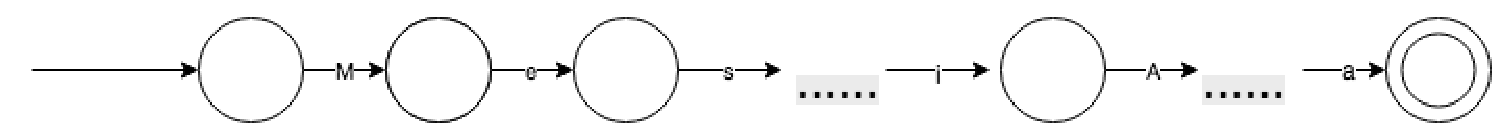
\includegraphics[scale=0.4]{lect3_img1.eps}
\end{unnumfigure}

$M_3$ accepts $L_1 \circ L_2$ $\Rightarrow$ $L_1 \circ L_2$ is regular.

\begin{definition}
    A \emph{non-deterministic finite automaton} is a 5-tuple $M = (Q, \Sigma, \delta, q_0, F)$ s.t.

    \begin{itemize}
        \item $Q, \Sigma, q_0, F$ are the same
        \item $\delta: Q \times (\Sigma \cup \{\epsilon\}) \rightarrow 2^Q$
        \begin{itemize}
            \item $\delta (q, s)$ is a subset of $Q$
        \end{itemize}
    \end{itemize}
\end{definition}

For a set $S$, $2^S$ is called the \emph{power set} of $S$. It contains all subsets of $S$.

$2^{\set{a, b}} = \set{\emptyset, \set{a}, \set{b}, \set{a, b}}$

\begin{definition}
    The NFA $M$ accepts the string  $w = w_1w_2 \ldots$ if there exists a string $y = y_1y_2 \ldots y_m \in (\Sigma \cup \set{\epsilon})^*$  and a sequence $r0, r_1, \ldots r_m \in Q$ such that:

    \begin{itemize}
        \item $w = y_1 \circ y_2 \circ \cdots \circ y_m$
        \item $r_0 = q_0$
        \item $r_i \in \delta (r_{i-1}, y_i) \text{ for } i = 1, \cdots, m$
        \item $r_m \in F$
    \end{itemize}
\end{definition}

Input string: $w = 00$

$y = \epsilon 00$, $r = q_0q_1q_2q_1$

$\delta(q_0, \epsilon) = \set{q_1, q_3}$

\backmatter
